\documentclass[12pt]{article}
\usepackage[a4paper, total={6.5in, 10in}]{geometry}

\usepackage{listings}
\usepackage{color}

\definecolor{dkgreen}{rgb}{0,0.6,0}
\definecolor{gray}{rgb}{0.5,0.5,0.5}
\definecolor{mauve}{rgb}{0.58,0,0.82}

\lstset{frame=tb,
  language=Haskell,
  aboveskip=3mm,
  belowskip=3mm,
  showstringspaces=false,
  columns=flexible,
  basicstyle={\small\ttfamily},
  numbers=none,
  numberstyle=\tiny\color{gray},
  keywordstyle=\color{blue},
  commentstyle=\color{dkgreen},
  stringstyle=\color{mauve},
  breaklines=true,
  breakatwhitespace=true,
  tabsize=3
}

\usepackage{amsmath}
\usepackage{amssymb}
\usepackage{enumitem}
\usepackage{braket}
\usepackage{qcircuit}
\usepackage{graphicx}

\newcommand{\code}{CS-IS-2010-1}
\newcommand{\name}{Midsemester Project Report}
\newcommand{\me}{Santripta Sharma}

\newcommand{\prob}[1]{\mathbb{P}\left[#1\right]}

\newcommand{\kz}{\ket{0}}
\newcommand{\ko}{\ket{1}}
\newcommand{\kp}{\ket{\phi}}
\newcommand{\ks}{\ket{\psi}}
\newcommand{\kso}{\ket{\psi_1}}
\newcommand{\kst}{\ket{\psi_2}}

\newcommand{\rec}[1]{\frac{1}{#1}}

\newenvironment*{qparts}{\begin{enumerate}[label=(\alph*)]}{\end{enumerate}}

\title{\code: \name}
\author{\me}
\date{\today}

\markright{\code\hspace{0.5in}\name\hspace{0.5in}\me}

\parindent=0pt

\begin{document}
\maketitle
\hrule \bigskip

\section{Problem Statement \& Requirements}
\subsection{Problem Statement}
Develop a classification model over the Iris Dataset and store the model. Then write a Haskell code to restore the model, input new data (based on the four features of the iris) and generate a prediction in real time.
\begin{enumerate}
	\item Input: The Iris Dataset.
	\item Output: Real-time prediction for the class of the flower of a new data row containing the sepal width, petal width, sepal length and petal length.
	\item Method: You can use Python to train and save a classification model (SVM or NN). However, restoring the model and the real-time prediction of a new data row has to be written only in Haskell.
\end{enumerate}

\subsection{Requirements}
Based on this problem statement, the project's requirements can be formulated as follows:
\begin{itemize}
	\item The system should be able to load a trained classification model.
	\item Given any new data point of the same format as the iris dataset by the user, the system should be able to use the loaded model to make a prediction on this data and report it to the user.
	\item The inference part of the system should be as performant as possible, since the problem description suggests that the application domain is a real-time system.
\end{itemize}

\section{Specification}
Generalising from the requirements, we offer the following featureset:
\begin{enumerate}
	\item Parsing capabilities to restore the shape, weights, and biases of \textbf{an arbitrary} FFN-based classifier from a file.
	\item Interactive \& batched modes of performing inference. \begin{itemize}
		\item \textbf{Interactive}: The user enters a single new datapoint and gets predictions for it in real-time. Structured as a Read-Eval-Print-Loop (REPL).
		\item \textbf{Batched}: The user provides many datapoints in a csv file, and receives predictions for each point. Additionally, the system reports aggregate statistics.
	\end{itemize}
\end{enumerate}
To briefly expand on point 1, since the type of model (FFN) is known, we can generalise the system to work with any classifier following that architecture, since this is independent of the particular dataset used, as long as that dataset only contains numeric feature. This allows the system to be reused for similar tasks beyond the Iris dataset.\bigskip

\begin{figure}
	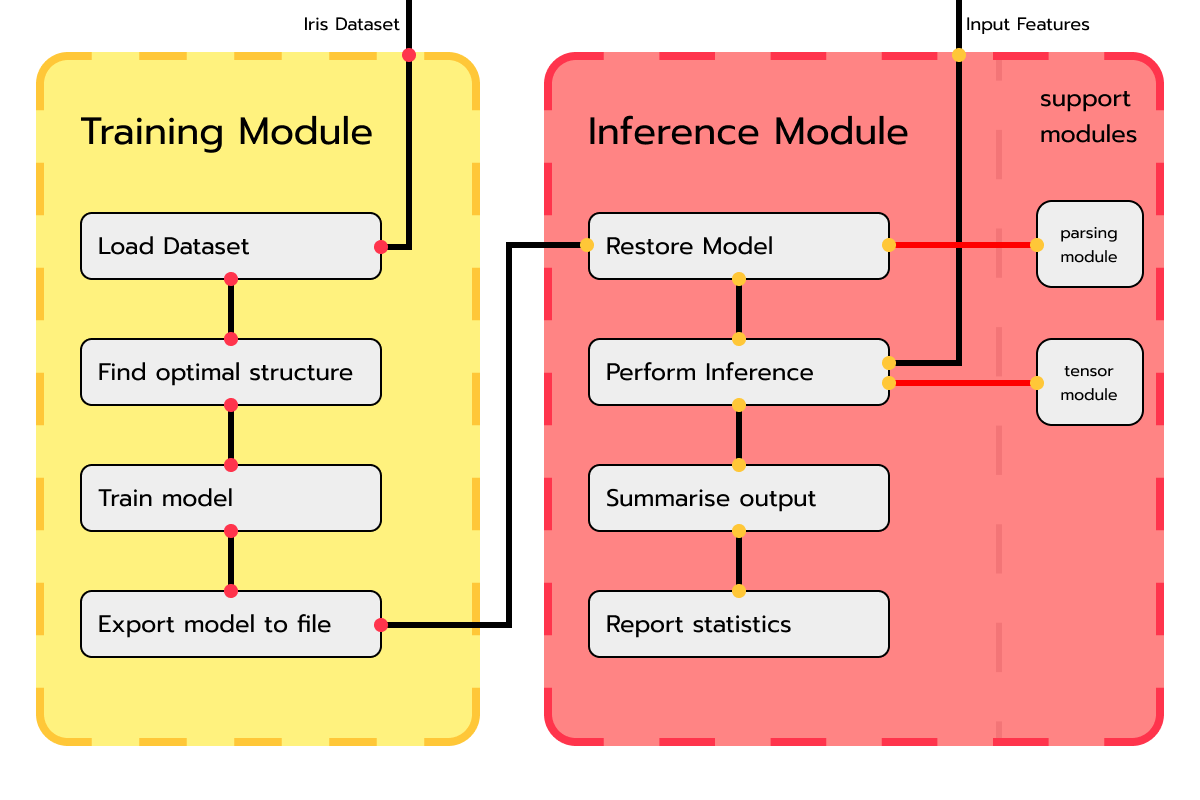
\includegraphics[width=0.85\pdfpagewidth]{../images/modules.png}
	\caption{the high-level architecture}
\end{figure}

\section{Design \& Architecture}
Since we are only concerned with running the inference for a new row for this dataset, we train our classification models separately (for testing purposes) before runtime. At runtime, we restore the structure, weights, and biases of the model, and push the given feature vector through the model in order to arrive at the inferred output.\bigskip

Then, the system can broadly be divided into two modules, the training module \& the inference module. These operate independently from each other, with the only interface between them being the inference module taking the training module's output (model structure, weights, biases) as its input, which is then used to reconstruct the model. Figure 1 illustrates the general flow of this design.\bigskip

First, we look at the common thread between the two modules, the file format for sharing the trained model parameters.

\subsection{Trained Model Format}
For the prototyping stage, we opt to use a plaintext format for the trained model parameters, since this allows easier debugging and editing.\bigskip

We know that a feedforward neural network is comprised of several layers of neurons, with each layer (besides the input layer) having a matrix of weights \& a vector of biases associated with itself. Further, using the propagation formula $Wx + b$, we can infer the incoming and outgoing dimension of each stage from these matrices alone.\bigskip

Then, our format is simply a text file structured as follows:
\begin{verbatim}
for each layer in the network:
    weights matrix
    biases vector
\end{verbatim}
For example, this is the model file for a network with a single hidden layer of size 5:
\begin{verbatim}
[[ 0.23400233  0.46448114 -0.18169046 -1.02006724]
[ 0.91292487 -0.83703552  0.46820428  1.07709024]
[ 0.77124784  0.60032112 -1.04011005 -1.06176582]
[ 0.04108179  0.0236362  -0.6077499  -0.57499983]
[ 0.41324034  0.71752045 -1.10962444  0.24183919]]
[ 1.05104845 -1.15333131  1.42181299  0.46979225 -0.31311588]
[[ 0.54906348 -1.2267044   1.117347   -0.7446324   1.17420772]
[-0.24563245 -0.00604219  1.02716034  0.51893559 -0.44818289]
[-0.79535198  0.72517445 -1.57061672  0.55235219  0.11317021]]
[ 0.18887961  0.43315065 -0.37568123]   
\end{verbatim}
From the first layer's weights having four columns, we can infer that there are four input features, and from the last layer's weights having three rows, we can infer that there are three output classes. This ability to infer input \& output shape at parse-time is what allows this structure to be independent of the dataset the model is trained for.\bigskip

It is also worth stating that the system currently makes the assumption that the network uses a ReLU activation at every layer except the last, where softmax is used (as is customary for multiclass classification). Therefore, in truth, the space of models the system accepts is a little more restricted than claimed in the specification (since in a classification model, the ReLU here could very well be replaced by a variety of alternative activation functions).\bigskip

We can now dissect the modules separately.

\subsection{Training Module}
The purpose of the training module is to provide us with a set of models we can use to test our inference module. As such, we don't strictly require a high performance model. However, we still perform some basic hyperparameter selection after loading the dataset in using a 5-fold cross validation approach to determine the shape of the network (number \& size of hidden layers).\bigskip

The model architecture used is the one mentioned above, a simple feedforward network, a sequence of linear layers using the ReLU activation function between the hidden layers, and the softmax activation at the end. Using a grid search, we find the top 5 performing shapes, and also one poorly performing shape, out of a generated set of possible shapes for the network.\bigskip

Before fitting 6 models using these shapes on the data, the data is transformed by converting the output classes column from textual labels to numerical labels, to avoid any ordering ambiguities arising during the training process. This transformed data is then split into. into training \& test sets, and fit the models on the training set.\bigskip

Finally, we write the networks' shapes, weights, and biases into model files, which can then be used by the inference module.

\subsection{Inference Module}
The inference module constitutes the bulk of the codebase. It produces an executable with the following signature:
\begin{verbatim}
inference-exe <path_to_model_file> [<path_to_batch_csv>]
\end{verbatim}
If the second, optional argument is omitted, it starts in interactive mode. Otherwise, it starts in batched mode.\bigskip

In either case, its first task is to restore the model from the given model file. Here, we utilise the parsing support module, which will be discussed in the Tooling section.\bigskip

Through this parsing process, the model shape, and its parameters are loaded into a data structure which takes the form of a list of layers, where each layer stores its input \& output shapes, and the weights \& biases matrices.\bigskip

Next, based on which mode it was started in, the system either enters a REPL or parses the input batch csv file it was provided (again, with the help of the parsing support module). In either mode, once the feature vector(s) are acquired, the tensor support module is used to perform the sequence of computations that lead to the final prediction.\bigskip

The final output (for each feature vector) is the predicted class and the probabilities associated with each class. In the case of batch mode, we also report summary statistics, how many vectors belonged to each class.

\section{Tooling}
\subsection{Training Module}
The training module is written in python, using numpy, pandas, and sklearn to perform the data processing \& model training/selection.\bigskip

\subsection{Inference Module}
The inference module is written in Haskell. We use the Haskell Tool Stack (or just Stack) as our build tool. The following dependencies are used:
\begin{itemize}
	\item \textbf{matrix \& vector}\\
	As the name suggests, these two packages provide a Matrix \& Vector type respectively, also providing the definitions for common mathematical operations on them, including matrix multiplication, converting between the two types, etc.\bigskip

	Together, they form the tensor support module, which is used to finally perform the inference once the inputs have been parsed.

	\item \textbf{parsec}\\
	Parsec is Haskell's standard parser combinator library, allowing us to write atomic parsers and compose them together. Parsec forms the foundations of the parsing support module, which is used for parsing both the model files \& csv files for batched input mode.\bigskip

	Discussion of the specifics of the parser implementations is deferred to the Prototype Details section.
\end{itemize}

\subsection{Testing/Miscellaneous}
A mix of bash \& python scripts is used to implement the end-to-end tests and certain convenient utilities (eg. infer.py for loading and making predictions using sklearn, used to verify infer module). 

\section{Test Plan}
Due to the large number of disjoint moving parts in the project, the plan is to implement a test suite consisting of unit \& end-to-end tests.

\subsection{Unit Testing}
First, we note that the training module does not require testing, due to its simplicity and it almost exclusively using sklearn library functions. For the inference module, all the parser functions, and many of the inference functions are complex enough to warrant unit testing. We plan to implement these using HSpec, which is the testing framework Stack provides.\bigskip

In order to cover the large space of inputs for these functions, we plan to heavily depend on generated test suites, as opposed to hand-crafted ones.

Consider two examples:
\begin{itemize}
	\item \textbf{For the matrix parser:} We generate random real-valued matrices, stringify them, run them through the parser, and verify that the same matrix is recovered.
	\item \textbf{For batch softmax:} Use single-vector inference softmax as oracle and verify batch softmax.
\end{itemize}

\subsection{End-to-End Testing}
We use an end-to-end test to verify the correctness of our inference module. Here, we treat our sklearn model as an oracle, randomly generating many batches of feature vectors (in addition to the existing test split), running them through both our oracle \& the inference module, and comparing the output activations.

\section{Prototype Details}
\subsection{Project Structure}
\begin{verbatim}
src
|
-- inference <--- inference module
|  |
|  -- app/Main.hs    <--- driver code
|  -- src/Lib.hs     <--- tensor support module
|  -- src/Parser.hs  <--- parsing support module
|  ...
-- models    <--- pickled sklearn models (for testing)
-- weights   <--- model files
-- infer.py  <--- sklearn inference helper
-- iris*.csv <--- datasets
-- train_model.ipynb <--- training module
\end{verbatim}

\subsection{Feature Set}
The prototype implements the following features:
\begin{itemize}
	\item Complete restoration of any feed-forward classifier, given its parameters in the model file format, assuming it uses ReLU + Softmax activations.
	\item Interactive mode REPL, where the user can enter new datapoints, and get prediction outputs (activations + class label) for them.
	\item Batch mode, where the user can provide a csv file of datapoints to run inference on, and get prediction outputs for each point.
\end{itemize}

\subsection{Limitations}
\begin{itemize}
	\item Lack of runtime checks for user input, leading to a restrictive input format \& several non-graceful exits, without any useful feedback to the user.
	\item Class of models that works limited to ReLU + Softmax activation based classifiers (large but not comprehensive).
	\item The csv input in batch mode can't end on a blank line (parser bug)
	\item Batch mode doesn't provide summary statistics
\end{itemize}

\subsection{Exploration of Selected Functionality}
\subsubsection{Parsing a model file}
The power of a parser combinator comes from its characteristic composability of various atomic parsers, which can each be individually tested, building up to the final parser. To illustrate this, here's the parser for a number within a model file.
\begin{lstlisting}
number :: Parser Double
number = do
	sign <- option "" $ string "-"
	int <- many1 digit <?> "integer part"
	dec <- option "" $ do
		void $ char '.'
		frac <- many1 digit
		return $ '.' : frac
	pow <- option "" $ do
		void $ char 'e'
		esign <- option "" $ string "-" <|> string "+"
		num <- many1 digit
		let epart = 'e':(esign ++ num)
		return epart
	let num = read (sign ++ int ++ dec ++ pow) :: Double
	return num	
\end{lstlisting}
This parser parses out a double-precision floating point number, given a string which may or may not be in scientific notation (eg. 2.35 vs 3.31045e-5). Once we are convinced about the correctness of this parser, perhaps by throwing test cases at it, we can use this parser to implement a parser for bias vectors:
\begin{lstlisting}
vector :: Parser [Double]
vector = do
	void $ char '['
	eatWhitespace
	numbers <- sepEndBy number (many1 whitespace)
	void (char ']' <?> "vector closing bracket")
	return numbers
\end{lstlisting}
Here, we have a parser which returns a list of doubles, essentially a vector. As we convince ourselves of its correctness through testing, it occurs to us that this parser can apply not only to bias vectors, but also to the vectors within each matrix. After all, matrices are represented as lists of vectors. Then, we arrive at a parser for matrices:
\begin{lstlisting}
matrix :: Parser (Matrix Double, Int, Int)
matrix = do
	void $ char '['
	eatWhitespace
	rows <- sepEndBy vector (many1 whitespace)
	void (char ']' <?> "matrix closing bracket")
	let nRows = length rows
	let nCols = length $ head rows
	return (Mat.fromList nRows nCols (concat rows), nRows, nCols)
\end{lstlisting}
And so on we go, composing our parsers all the way up the chain until we have a fully functional model file parser. It is hard to overstate the convenience and confidence this approach of writing a parser provides, where we can incrementally test each stage of our parser, using it as a foundation for the next layer.

\subsubsection{Batch inference}
As a prerequisite for this section, here's what the network data structure looks like:
\begin{lstlisting}
type Network = [Layer]

data Layer = Layer {
		inDim :: Int,
		outDim :: Int,
		weights :: Matrix Double,
		biases :: Matrix Double
	}
\end{lstlisting}
Quite simply, a feed-forward neural network can be modeled as a list of layers. Now, to perform inference of a single vector on this network, we have:
\begin{lstlisting}
inferSingle :: Network -> Vector Double -> Vector Double
inferSingle net input = getCol 1 $ softLayer 
			(foldl reluLayer inpMat nonLinear) final
	where
		inpMat = colVector input
		size = length net
		nonLinear = take (size - 1) net
		final = last net

		inferLayer :: Matrix Double -> Layer -> Matrix Double
		inferLayer inp (Layer _ _ w b) = w * inp + b

		reluLayer :: Matrix Double -> Layer -> Matrix Double
		reluLayer inp lay = relu (inferLayer inp lay)

		softLayer :: Matrix Double -> Layer -> Matrix Double
		softLayer inp lay = softmax (inferLayer inp lay)
\end{lstlisting}
Assuming that \verb|relu| \& \verb|softmax| are easy to define (they are), this is a fairly simple construction. So, then, since the inferLayer function is already using matrices under the hood, and matrix multiplication distributes under column concatenation, surely batch inference is a simple extension, like so:
\begin{lstlisting}
inferBatch :: Network -> Matrix Double -> Matrix Double
inferBatch net input = softLayer (foldl reluLayer input nonLinear) final
	where
		size = length net
		nonLinear = take (size - 1) net
		final = last net

		inferLayer :: Matrix Double -> Layer -> Matrix Double
		inferLayer inp (Layer _ _ w b) = w * inp + b
		...
\end{lstlisting}
Seems simple enough, and it compiles as well, so this must work, surely?

Of course not, batchInference fails with a distinctly obtuse runtime error that fails to even provide a proper call stack. After a little bit of exploration, it becomes clear that the bias dimensions no longer match, since $Wx$ now has multiple columns, but $b$ retains only one column, making $Wx + b$ incoherent. Easy enough fix:
\begin{lstlisting}
inferBatch :: Network -> Matrix Double -> Matrix Double
inferBatch net input = softLayer (foldl reluLayer input nonLinear) final
	where
		size = length net
		nonLinear = take (size - 1) net
		final = last net

		inputCols = ncols input

        expandCols :: Matrix Double -> Matrix Double
        expandCols mat = foldr (\_ acc -> acc <|> mat) mat [1..inputCols]

		inferLayer :: Matrix Double -> Layer -> Matrix Double
		inferLayer inp (Layer _ _ w b) = w * inp + (expandCols b)
		...
\end{lstlisting}
And this does solve the error, opening the gates to another, more subtle error. The batch inference is producing results, but the output activations don't look much like probabilities, as they should after a softmax.\bigskip

Upon investigating the softmax implementation, the cause becomes clear:
\begin{lstlisting}
softmax :: Matrix Double -> Matrix Double
softmax v = (/ denom) . exp <$> v
			where denom = sum (exp <$> v)	
\end{lstlisting}
This works perfectly fine, when there is exactly one column in the matrix (the argument name itself, captures much of the reason for this incorrectness). When this is not the case, however, the denominator is accumulated over all elements of the matrix, instead of per output vector. Therefore, we need to generalise this single column softmax function to a multi column soft max function. Unfortunately, due to the minimal interface of the matrix package, the cleanest solution I have currently been able to come up for this is:
\begin{lstlisting}
batchSoftmax :: Matrix Double -> Matrix Double
batchSoftmax mat = submatrix 1 rows 1 inputCols (foldr folder (fromList rows 1 [1..]) [1..inputCols])
	where
		rows = nrows mat
		folder :: Int -> Matrix Double -> Matrix Double
		folder colIdx acc = colVector ((/ denom col) . exp <$> col) <|> acc
			where col = getCol colIdx mat

		denom :: Vector Double -> Double
		denom col = sum (exp <$> col)
\end{lstlisting}

\section{Plan for Completion}
A high-level roadmap for the project's completion is as follows:
\begin{itemize}
	\item Perform runtime checks on input dimension during inference.
	\item Runtime checks for interactive mode (for graceful fails).
	\item Implement the test suite discussed above.
	\item Allow alternative activation functions for non-output layers, as opposed to assuming ReLU.
	\item Add testing mode, given batch and expected outputs, report model accuracy.
	\item Add aggregation mode, use multiple trained models with voting (ensemble method).
\end{itemize}
Upon delivery of all these tasks, the project will be in its completed state.\bigskip

The choice to develop tests \& more robust runtime checks for the existing features before moving onto the new features is so that I can gain a better understanding of how to structure exception handling in haskell, and also learn how to use HSpec for unit tests. Then, as the new features are being implemented, a test-driven approach can be followed, allowing the new features to be verified as they're implemented.

\end{document}